\documentclass[twoside]{book}

% Packages required by doxygen
\usepackage{fixltx2e}
\usepackage{calc}
\usepackage{doxygen}
\usepackage[export]{adjustbox} % also loads graphicx
\usepackage{graphicx}
\usepackage[utf8]{inputenc}
\usepackage{makeidx}
\usepackage{multicol}
\usepackage{multirow}
\PassOptionsToPackage{warn}{textcomp}
\usepackage{textcomp}
\usepackage[nointegrals]{wasysym}
\usepackage[table]{xcolor}

% Font selection
\usepackage[T1]{fontenc}
\usepackage[scaled=.90]{helvet}
\usepackage{courier}
\usepackage{amssymb}
\usepackage{sectsty}
\renewcommand{\familydefault}{\sfdefault}
\allsectionsfont{%
  \fontseries{bc}\selectfont%
  \color{darkgray}%
}
\renewcommand{\DoxyLabelFont}{%
  \fontseries{bc}\selectfont%
  \color{darkgray}%
}
\newcommand{\+}{\discretionary{\mbox{\scriptsize$\hookleftarrow$}}{}{}}

% Page & text layout
\usepackage{geometry}
\geometry{%
  a4paper,%
  top=2.5cm,%
  bottom=2.5cm,%
  left=2.5cm,%
  right=2.5cm%
}
\tolerance=750
\hfuzz=15pt
\hbadness=750
\setlength{\emergencystretch}{15pt}
\setlength{\parindent}{0cm}
\setlength{\parskip}{3ex plus 2ex minus 2ex}
\makeatletter
\renewcommand{\paragraph}{%
  \@startsection{paragraph}{4}{0ex}{-1.0ex}{1.0ex}{%
    \normalfont\normalsize\bfseries\SS@parafont%
  }%
}
\renewcommand{\subparagraph}{%
  \@startsection{subparagraph}{5}{0ex}{-1.0ex}{1.0ex}{%
    \normalfont\normalsize\bfseries\SS@subparafont%
  }%
}
\makeatother

% Headers & footers
\usepackage{fancyhdr}
\pagestyle{fancyplain}
\fancyhead[LE]{\fancyplain{}{\bfseries\thepage}}
\fancyhead[CE]{\fancyplain{}{}}
\fancyhead[RE]{\fancyplain{}{\bfseries\leftmark}}
\fancyhead[LO]{\fancyplain{}{\bfseries\rightmark}}
\fancyhead[CO]{\fancyplain{}{}}
\fancyhead[RO]{\fancyplain{}{\bfseries\thepage}}
\fancyfoot[LE]{\fancyplain{}{}}
\fancyfoot[CE]{\fancyplain{}{}}
\fancyfoot[RE]{\fancyplain{}{\bfseries\scriptsize Generated by Doxygen }}
\fancyfoot[LO]{\fancyplain{}{\bfseries\scriptsize Generated by Doxygen }}
\fancyfoot[CO]{\fancyplain{}{}}
\fancyfoot[RO]{\fancyplain{}{}}
\renewcommand{\footrulewidth}{0.4pt}
\renewcommand{\chaptermark}[1]{%
  \markboth{#1}{}%
}
\renewcommand{\sectionmark}[1]{%
  \markright{\thesection\ #1}%
}

% Indices & bibliography
\usepackage{natbib}
\usepackage[titles]{tocloft}
\setcounter{tocdepth}{3}
\setcounter{secnumdepth}{5}
\makeindex

% Hyperlinks (required, but should be loaded last)
\usepackage{ifpdf}
\ifpdf
  \usepackage[pdftex,pagebackref=true]{hyperref}
\else
  \usepackage[ps2pdf,pagebackref=true]{hyperref}
\fi
\hypersetup{%
  colorlinks=true,%
  linkcolor=blue,%
  citecolor=blue,%
  unicode%
}

% Custom commands
\newcommand{\clearemptydoublepage}{%
  \newpage{\pagestyle{empty}\cleardoublepage}%
}

\usepackage{caption}
\captionsetup{labelsep=space,justification=centering,font={bf},singlelinecheck=off,skip=4pt,position=top}

%===== C O N T E N T S =====

\begin{document}

% Titlepage & ToC
\hypersetup{pageanchor=false,
             bookmarksnumbered=true,
             pdfencoding=unicode
            }
\pagenumbering{roman}
\begin{titlepage}
\vspace*{7cm}
\begin{center}%
{\Large Simulation \\[1ex]\large 2.\+01 }\\
\vspace*{1cm}
{\large Generated by Doxygen 1.8.11}\\
\end{center}
\end{titlepage}
\clearemptydoublepage
\tableofcontents
\clearemptydoublepage
\pagenumbering{arabic}
\hypersetup{pageanchor=true}

%--- Begin generated contents ---
\chapter{Hierarchical Index}
\section{Class Hierarchy}
This inheritance list is sorted roughly, but not completely, alphabetically\+:\begin{DoxyCompactList}
\item \contentsline{section}{sim.\+Run}{\pageref{classsim_1_1_run}}{}
\item Runnable\begin{DoxyCompactList}
\item \contentsline{section}{sim.\+Field}{\pageref{classsim_1_1_field}}{}
\end{DoxyCompactList}
\item J\+Component\begin{DoxyCompactList}
\item \contentsline{section}{sim.\+Field}{\pageref{classsim_1_1_field}}{}
\end{DoxyCompactList}
\item J\+Frame\begin{DoxyCompactList}
\item \contentsline{section}{sim.\+Window}{\pageref{classsim_1_1_window}}{}
\end{DoxyCompactList}
\end{DoxyCompactList}

\chapter{Class Index}
\section{Class List}
Here are the classes, structs, unions and interfaces with brief descriptions\+:\begin{DoxyCompactList}
\item\contentsline{section}{\hyperlink{classsim_1_1_field}{sim.\+Field} }{\pageref{classsim_1_1_field}}{}
\item\contentsline{section}{\hyperlink{classsim_1_1_run}{sim.\+Run} }{\pageref{classsim_1_1_run}}{}
\item\contentsline{section}{\hyperlink{classsim_1_1_window}{sim.\+Window} }{\pageref{classsim_1_1_window}}{}
\end{DoxyCompactList}

\chapter{Class Documentation}
\hypertarget{classsim_1_1_field}{}\section{sim.\+Field Class Reference}
\label{classsim_1_1_field}\index{sim.\+Field@{sim.\+Field}}
Inheritance diagram for sim.\+Field\+:\begin{figure}[H]
\begin{center}
\leavevmode
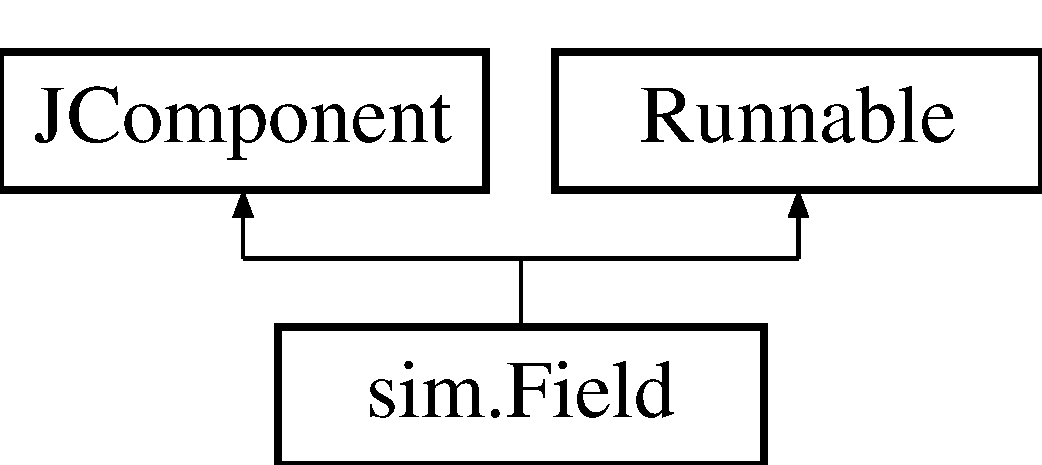
\includegraphics[height=2.000000cm]{classsim_1_1_field}
\end{center}
\end{figure}
\subsection*{Public Member Functions}
\begin{DoxyCompactItemize}
\item 
void \hyperlink{classsim_1_1_field_a6a42c9b7dfcbb948ccf89351358575fd}{set\+Speed} (int speed)
\item 
void \hyperlink{classsim_1_1_field_abeb32b6171955cae5e65a1c2f0d9819a}{set\+Colour\+Change\+Chance} (double chance)
\item 
int \hyperlink{classsim_1_1_field_aacac61a31d2b8da325e306f4040e7929}{get\+Speed} ()
\item 
void \hyperlink{classsim_1_1_field_af65ffe349f271f67977fa98707711908}{set\+Neighbour} (\hyperlink{classsim_1_1_field}{Field} neighbour)
\item 
Color \hyperlink{classsim_1_1_field_a5ad0b86ec796915ff1588c37937b58b6}{get\+Colour} ()
\item 
void \hyperlink{classsim_1_1_field_ae0f6d5b684a2cc8800a6cf6c3763cad3}{change\+Colour} ()
\item 
void \hyperlink{classsim_1_1_field_a4efbcf3a218e4aa1ef448ce7b145e0a2}{Schedule\+Field} ()
\item 
void \hyperlink{classsim_1_1_field_a1d7072dab1f7a54d9ca0698e03edb6b6}{Stop\+Field} ()
\item 
\hyperlink{classsim_1_1_field_ae7740288b2977c923876876936a8a3e7}{Field} (Random rand, double colour\+\_\+change\+\_\+chance, int speed, Reentrant\+Lock super\+\_\+lock)  throws Illegal\+Argument\+Exception
\item 
void {\bfseries run} ()\hypertarget{classsim_1_1_field_a45d95ea1b7811cafdc14d0f0a79385d8}{}\label{classsim_1_1_field_a45d95ea1b7811cafdc14d0f0a79385d8}

\end{DoxyCompactItemize}
\subsection*{Public Attributes}
\begin{DoxyCompactItemize}
\item 
Read\+Write\+Lock \hyperlink{classsim_1_1_field_a6f067507d7109db5ec9f1bcb967c9a8c}{lock}
\end{DoxyCompactItemize}
\subsection*{Protected Member Functions}
\begin{DoxyCompactItemize}
\item 
void {\bfseries paint\+Component} (Graphics g)\hypertarget{classsim_1_1_field_a3cab9d793a3f7d165b6ce8b78dbf7c9a}{}\label{classsim_1_1_field_a3cab9d793a3f7d165b6ce8b78dbf7c9a}

\end{DoxyCompactItemize}


\subsection{Detailed Description}
Class of field that changes its colour depending on neighbours or at random. To Start chaning it needs to be executed at fixed rate, best at \hyperlink{classsim_1_1_field_aacac61a31d2b8da325e306f4040e7929}{get\+Speed()} speed. \begin{DoxyAuthor}{Author}
n1t4chi 
\end{DoxyAuthor}


\subsection{Constructor \& Destructor Documentation}
\index{sim\+::\+Field@{sim\+::\+Field}!Field@{Field}}
\index{Field@{Field}!sim\+::\+Field@{sim\+::\+Field}}
\subsubsection[{\texorpdfstring{Field(\+Random rand, double colour\+\_\+change\+\_\+chance, int speed, Reentrant\+Lock super\+\_\+lock)}{Field(Random rand, double colour_change_chance, int speed, ReentrantLock super_lock)}}]{\setlength{\rightskip}{0pt plus 5cm}sim.\+Field.\+Field (
\begin{DoxyParamCaption}
\item[{Random}]{rand, }
\item[{double}]{colour\+\_\+change\+\_\+chance, }
\item[{int}]{speed, }
\item[{Reentrant\+Lock}]{super\+\_\+lock}
\end{DoxyParamCaption}
) throws Illegal\+Argument\+Exception}\hypertarget{classsim_1_1_field_ae7740288b2977c923876876936a8a3e7}{}\label{classsim_1_1_field_ae7740288b2977c923876876936a8a3e7}
Constructor. 
\begin{DoxyParams}{Parameters}
{\em rand} & R\+NG. \mbox{[}must not be null pointer\mbox{]} \\
\hline
{\em colour\+\_\+change\+\_\+chance} & chance of field changing its colour randomly. \mbox{[}must be positive\mbox{]} \\
\hline
{\em speed} & Speed of changing colour. \mbox{[}must be within \mbox{[}0,1\mbox{]} range\mbox{]} \\
\hline
{\em super\+\_\+lock} & Super lock when all fields properties are being changed. \\
\hline
\end{DoxyParams}

\begin{DoxyExceptions}{Exceptions}
{\em Illegal\+Argument\+Exception} & if given arguments are not correct. \\
\hline
\end{DoxyExceptions}


\subsection{Member Function Documentation}
\index{sim\+::\+Field@{sim\+::\+Field}!change\+Colour@{change\+Colour}}
\index{change\+Colour@{change\+Colour}!sim\+::\+Field@{sim\+::\+Field}}
\subsubsection[{\texorpdfstring{change\+Colour()}{changeColour()}}]{\setlength{\rightskip}{0pt plus 5cm}void sim.\+Field.\+change\+Colour (
\begin{DoxyParamCaption}
{}
\end{DoxyParamCaption}
)}\hypertarget{classsim_1_1_field_ae0f6d5b684a2cc8800a6cf6c3763cad3}{}\label{classsim_1_1_field_ae0f6d5b684a2cc8800a6cf6c3763cad3}
Changes colour of this field, either randomly or from average neighbour colour. \index{sim\+::\+Field@{sim\+::\+Field}!get\+Colour@{get\+Colour}}
\index{get\+Colour@{get\+Colour}!sim\+::\+Field@{sim\+::\+Field}}
\subsubsection[{\texorpdfstring{get\+Colour()}{getColour()}}]{\setlength{\rightskip}{0pt plus 5cm}Color sim.\+Field.\+get\+Colour (
\begin{DoxyParamCaption}
{}
\end{DoxyParamCaption}
)}\hypertarget{classsim_1_1_field_a5ad0b86ec796915ff1588c37937b58b6}{}\label{classsim_1_1_field_a5ad0b86ec796915ff1588c37937b58b6}
Returns current colour. \begin{DoxyReturn}{Returns}
Current colour. 
\end{DoxyReturn}
\index{sim\+::\+Field@{sim\+::\+Field}!get\+Speed@{get\+Speed}}
\index{get\+Speed@{get\+Speed}!sim\+::\+Field@{sim\+::\+Field}}
\subsubsection[{\texorpdfstring{get\+Speed()}{getSpeed()}}]{\setlength{\rightskip}{0pt plus 5cm}int sim.\+Field.\+get\+Speed (
\begin{DoxyParamCaption}
{}
\end{DoxyParamCaption}
)}\hypertarget{classsim_1_1_field_aacac61a31d2b8da325e306f4040e7929}{}\label{classsim_1_1_field_aacac61a31d2b8da325e306f4040e7929}
Returns speed of this field \mbox{[}in miliseconds\mbox{]}. \begin{DoxyReturn}{Returns}
speed of this field. 
\end{DoxyReturn}
\index{sim\+::\+Field@{sim\+::\+Field}!Schedule\+Field@{Schedule\+Field}}
\index{Schedule\+Field@{Schedule\+Field}!sim\+::\+Field@{sim\+::\+Field}}
\subsubsection[{\texorpdfstring{Schedule\+Field()}{ScheduleField()}}]{\setlength{\rightskip}{0pt plus 5cm}void sim.\+Field.\+Schedule\+Field (
\begin{DoxyParamCaption}
{}
\end{DoxyParamCaption}
)}\hypertarget{classsim_1_1_field_a4efbcf3a218e4aa1ef448ce7b145e0a2}{}\label{classsim_1_1_field_a4efbcf3a218e4aa1ef448ce7b145e0a2}
Schedules this thread for repeated execution \index{sim\+::\+Field@{sim\+::\+Field}!set\+Colour\+Change\+Chance@{set\+Colour\+Change\+Chance}}
\index{set\+Colour\+Change\+Chance@{set\+Colour\+Change\+Chance}!sim\+::\+Field@{sim\+::\+Field}}
\subsubsection[{\texorpdfstring{set\+Colour\+Change\+Chance(double chance)}{setColourChangeChance(double chance)}}]{\setlength{\rightskip}{0pt plus 5cm}void sim.\+Field.\+set\+Colour\+Change\+Chance (
\begin{DoxyParamCaption}
\item[{double}]{chance}
\end{DoxyParamCaption}
)}\hypertarget{classsim_1_1_field_abeb32b6171955cae5e65a1c2f0d9819a}{}\label{classsim_1_1_field_abeb32b6171955cae5e65a1c2f0d9819a}
Sets new random colour change chance. 
\begin{DoxyParams}{Parameters}
{\em chance} & New random colour change chance. \\
\hline
\end{DoxyParams}
\index{sim\+::\+Field@{sim\+::\+Field}!set\+Neighbour@{set\+Neighbour}}
\index{set\+Neighbour@{set\+Neighbour}!sim\+::\+Field@{sim\+::\+Field}}
\subsubsection[{\texorpdfstring{set\+Neighbour(\+Field neighbour)}{setNeighbour(Field neighbour)}}]{\setlength{\rightskip}{0pt plus 5cm}void sim.\+Field.\+set\+Neighbour (
\begin{DoxyParamCaption}
\item[{{\bf Field}}]{neighbour}
\end{DoxyParamCaption}
)}\hypertarget{classsim_1_1_field_af65ffe349f271f67977fa98707711908}{}\label{classsim_1_1_field_af65ffe349f271f67977fa98707711908}
Adds new neighbour. 
\begin{DoxyParams}{Parameters}
{\em neighbour} & New neighbour. \\
\hline
\end{DoxyParams}
\index{sim\+::\+Field@{sim\+::\+Field}!set\+Speed@{set\+Speed}}
\index{set\+Speed@{set\+Speed}!sim\+::\+Field@{sim\+::\+Field}}
\subsubsection[{\texorpdfstring{set\+Speed(int speed)}{setSpeed(int speed)}}]{\setlength{\rightskip}{0pt plus 5cm}void sim.\+Field.\+set\+Speed (
\begin{DoxyParamCaption}
\item[{int}]{speed}
\end{DoxyParamCaption}
)}\hypertarget{classsim_1_1_field_a6a42c9b7dfcbb948ccf89351358575fd}{}\label{classsim_1_1_field_a6a42c9b7dfcbb948ccf89351358575fd}
Sets new random speed of this field within range of \mbox{[}s/2 , 3/2$\ast$s\mbox{]}, where s is given average speed. 
\begin{DoxyParams}{Parameters}
{\em speed} & Average speed. \\
\hline
\end{DoxyParams}
\index{sim\+::\+Field@{sim\+::\+Field}!Stop\+Field@{Stop\+Field}}
\index{Stop\+Field@{Stop\+Field}!sim\+::\+Field@{sim\+::\+Field}}
\subsubsection[{\texorpdfstring{Stop\+Field()}{StopField()}}]{\setlength{\rightskip}{0pt plus 5cm}void sim.\+Field.\+Stop\+Field (
\begin{DoxyParamCaption}
{}
\end{DoxyParamCaption}
)}\hypertarget{classsim_1_1_field_a1d7072dab1f7a54d9ca0698e03edb6b6}{}\label{classsim_1_1_field_a1d7072dab1f7a54d9ca0698e03edb6b6}
Stops this field. 

\subsection{Member Data Documentation}
\index{sim\+::\+Field@{sim\+::\+Field}!lock@{lock}}
\index{lock@{lock}!sim\+::\+Field@{sim\+::\+Field}}
\subsubsection[{\texorpdfstring{lock}{lock}}]{\setlength{\rightskip}{0pt plus 5cm}Read\+Write\+Lock sim.\+Field.\+lock}\hypertarget{classsim_1_1_field_a6f067507d7109db5ec9f1bcb967c9a8c}{}\label{classsim_1_1_field_a6f067507d7109db5ec9f1bcb967c9a8c}
Lock for reading/writing. 

The documentation for this class was generated from the following file\+:\begin{DoxyCompactItemize}
\item 
src/sim/Field.\+java\end{DoxyCompactItemize}

\hypertarget{classsim_1_1_run}{}\section{sim.\+Run Class Reference}
\label{classsim_1_1_run}\index{sim.\+Run@{sim.\+Run}}
\subsection*{Static Public Member Functions}
\begin{DoxyCompactItemize}
\item 
static final void \hyperlink{classsim_1_1_run_a8cc89caa27b8800a57c34c3841f8d88f}{error} (String message)
\item 
static final void \hyperlink{classsim_1_1_run_a9326a45b817c0a7ad2b7c8f34f566fff}{print} (String message)
\item 
static final void \hyperlink{classsim_1_1_run_ad79f0200e37466cda3861593be66b0b2}{println} (String message)
\item 
static void \hyperlink{classsim_1_1_run_a1865b6bff5d8ffcf80dabeffc0ae3cbb}{main} (String\mbox{[}$\,$\mbox{]} args)
\end{DoxyCompactItemize}


\subsection{Detailed Description}
Main class that starts whole application. \begin{DoxyAuthor}{Author}
n1t4chi 
\end{DoxyAuthor}


\subsection{Member Function Documentation}
\index{sim\+::\+Run@{sim\+::\+Run}!error@{error}}
\index{error@{error}!sim\+::\+Run@{sim\+::\+Run}}
\subsubsection[{\texorpdfstring{error(\+String message)}{error(String message)}}]{\setlength{\rightskip}{0pt plus 5cm}static final void sim.\+Run.\+error (
\begin{DoxyParamCaption}
\item[{String}]{message}
\end{DoxyParamCaption}
)\hspace{0.3cm}{\ttfamily [static]}}\hypertarget{classsim_1_1_run_a8cc89caa27b8800a57c34c3841f8d88f}{}\label{classsim_1_1_run_a8cc89caa27b8800a57c34c3841f8d88f}
Prints error message if messages should be displayed 
\begin{DoxyParams}{Parameters}
{\em message} & Message to be displayed. \\
\hline
\end{DoxyParams}
\index{sim\+::\+Run@{sim\+::\+Run}!main@{main}}
\index{main@{main}!sim\+::\+Run@{sim\+::\+Run}}
\subsubsection[{\texorpdfstring{main(\+String[] args)}{main(String[] args)}}]{\setlength{\rightskip}{0pt plus 5cm}static void sim.\+Run.\+main (
\begin{DoxyParamCaption}
\item[{String\mbox{[}$\,$\mbox{]}}]{args}
\end{DoxyParamCaption}
)\hspace{0.3cm}{\ttfamily [static]}}\hypertarget{classsim_1_1_run_a1865b6bff5d8ffcf80dabeffc0ae3cbb}{}\label{classsim_1_1_run_a1865b6bff5d8ffcf80dabeffc0ae3cbb}
Main method. Runs \hyperlink{classsim_1_1_window}{Window}. Requires 4 \mbox{[}can be 5, more will be ignored\mbox{]} parameters as stated below\+: ~\newline
 1st argument\+: positive integer for amount of rows to be displayed. ~\newline
 2nd argument\+: positive integer for amount of columns to be displayed. ~\newline
 3rd argument\+: positive integer for speed \mbox{[}in miliseconds\mbox{]} of changing colour. ~\newline
 4th argument\+: double within range of \mbox{[}0,1\mbox{]} for chance of field changing colour randomly. ~\newline
 5th argument\mbox{[}optional\mbox{]}\+: if T\+R\+UE \mbox{[}case insensitive\mbox{]} information about colour changing will be displayed.~\newline
 
\begin{DoxyParams}{Parameters}
{\em args} & Arguments. \\
\hline
\end{DoxyParams}
\index{sim\+::\+Run@{sim\+::\+Run}!print@{print}}
\index{print@{print}!sim\+::\+Run@{sim\+::\+Run}}
\subsubsection[{\texorpdfstring{print(\+String message)}{print(String message)}}]{\setlength{\rightskip}{0pt plus 5cm}static final void sim.\+Run.\+print (
\begin{DoxyParamCaption}
\item[{String}]{message}
\end{DoxyParamCaption}
)\hspace{0.3cm}{\ttfamily [static]}}\hypertarget{classsim_1_1_run_a9326a45b817c0a7ad2b7c8f34f566fff}{}\label{classsim_1_1_run_a9326a45b817c0a7ad2b7c8f34f566fff}
Prints message if messages should be displayed 
\begin{DoxyParams}{Parameters}
{\em message} & Message to be displayed. \\
\hline
\end{DoxyParams}
\index{sim\+::\+Run@{sim\+::\+Run}!println@{println}}
\index{println@{println}!sim\+::\+Run@{sim\+::\+Run}}
\subsubsection[{\texorpdfstring{println(\+String message)}{println(String message)}}]{\setlength{\rightskip}{0pt plus 5cm}static final void sim.\+Run.\+println (
\begin{DoxyParamCaption}
\item[{String}]{message}
\end{DoxyParamCaption}
)\hspace{0.3cm}{\ttfamily [static]}}\hypertarget{classsim_1_1_run_ad79f0200e37466cda3861593be66b0b2}{}\label{classsim_1_1_run_ad79f0200e37466cda3861593be66b0b2}
Prints message if messages should be displayed. Adds line break. 
\begin{DoxyParams}{Parameters}
{\em message} & Message to be displayed. \\
\hline
\end{DoxyParams}


The documentation for this class was generated from the following file\+:\begin{DoxyCompactItemize}
\item 
src/sim/Run.\+java\end{DoxyCompactItemize}

\hypertarget{classsim_1_1_window}{}\section{sim.\+Window Class Reference}
\label{classsim_1_1_window}\index{sim.\+Window@{sim.\+Window}}
Inheritance diagram for sim.\+Window\+:\begin{figure}[H]
\begin{center}
\leavevmode
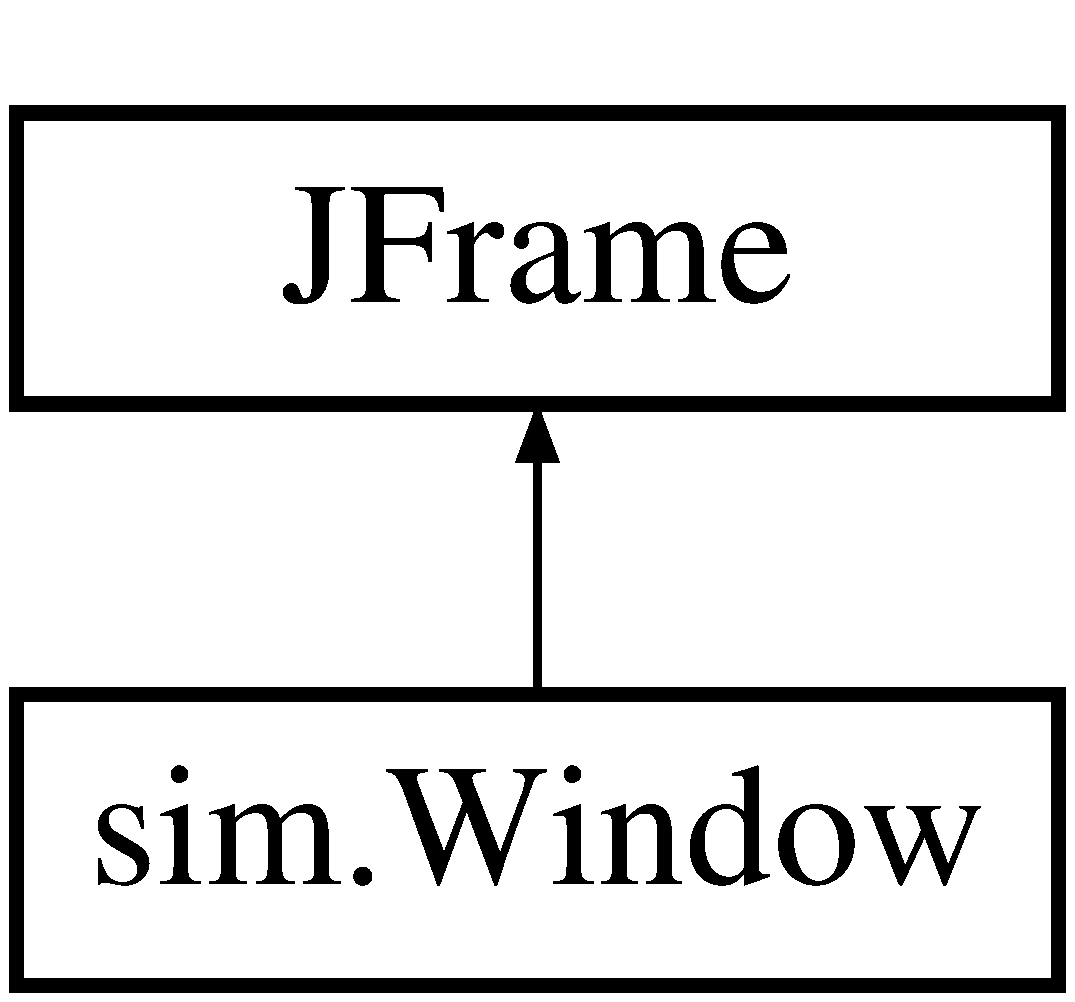
\includegraphics[height=2.000000cm]{classsim_1_1_window}
\end{center}
\end{figure}
\subsection*{Public Member Functions}
\begin{DoxyCompactItemize}
\item 
\hyperlink{classsim_1_1_window_ac192bb42f8dadb908135fec3ea5076ce}{Window} (int rows, int columns, int speed, double colour\+\_\+change\+\_\+chance)  throws Headless\+Exception,\+Illegal\+Argument\+Exception 
\end{DoxyCompactItemize}


\subsection{Detailed Description}
\hyperlink{classsim_1_1_window}{Window} class that displays fields. \begin{DoxyAuthor}{Author}
n1t4chi 
\end{DoxyAuthor}


\subsection{Constructor \& Destructor Documentation}
\index{sim\+::\+Window@{sim\+::\+Window}!Window@{Window}}
\index{Window@{Window}!sim\+::\+Window@{sim\+::\+Window}}
\subsubsection[{\texorpdfstring{Window(int rows, int columns, int speed, double colour\+\_\+change\+\_\+chance)}{Window(int rows, int columns, int speed, double colour_change_chance)}}]{\setlength{\rightskip}{0pt plus 5cm}sim.\+Window.\+Window (
\begin{DoxyParamCaption}
\item[{int}]{rows, }
\item[{int}]{columns, }
\item[{int}]{speed, }
\item[{double}]{colour\+\_\+change\+\_\+chance}
\end{DoxyParamCaption}
) throws Headless\+Exception,Illegal\+Argument\+Exception}\hypertarget{classsim_1_1_window_ac192bb42f8dadb908135fec3ea5076ce}{}\label{classsim_1_1_window_ac192bb42f8dadb908135fec3ea5076ce}
Constructor 
\begin{DoxyParams}{Parameters}
{\em rows} & amount of rows. \mbox{[}must be positive\mbox{]} \\
\hline
{\em columns} & amount of columns.\mbox{[}must be positive\mbox{]} \\
\hline
{\em speed} & speed of colour changing.\mbox{[}must be positive\mbox{]} \\
\hline
{\em colour\+\_\+change\+\_\+chance} & chance of field changing its colour randomly. \mbox{[}must be within \mbox{[}0,1\mbox{]} range\mbox{]} \\
\hline
\end{DoxyParams}

\begin{DoxyExceptions}{Exceptions}
{\em Headless\+Exception} & if system does not support G\+UI application. \\
\hline
{\em Illegal\+Argument\+Exception} & if given arguments are not correct. \\
\hline
\end{DoxyExceptions}


The documentation for this class was generated from the following file\+:\begin{DoxyCompactItemize}
\item 
src/sim/Window.\+java\end{DoxyCompactItemize}

%--- End generated contents ---

% Index
\backmatter
\newpage
\phantomsection
\clearemptydoublepage
\addcontentsline{toc}{chapter}{Index}
\printindex

\end{document}
